\section{Obbiettivo}

RIEMPIMI

\section{Ambiente di Lavoro}

Questa esercitazione \`{e} stata svolta all'interno del seguente ambiente di lavoro:

\begin{itemize}
	\item \textbf{Hardware}: 
		\begin{itemize}
			\item \textbf{CPU}: AMD Ryzen 9 5900x
			\item \textbf{RAM}: 32 GB DDR4 @3200 MHz
		\end{itemize}
	\item \textbf{Software}:
		\begin{itemize}
			\item \textbf{Host OS:} Arch Linux
			\item \textbf{Guest OS}: Ubuntu 20.4 LTS Server
			\item \textbf{Virtualization Software}: VirtualBox 6.1
		\end{itemize}
\end{itemize}

\section{Configurazione Macchine}

Per questa esercitazione sono necessarie 3 macchine virtuali che saranno 1 \lstinline[style=cmd]|master|, il quale avr\`{a} il compito di accettare i job e di effettuare lo scheduling di questi e 2 \lstinline[style=cmd]|slave| che avranno il compito di eseguire i vari job assegnategli . Ogni macchina \`{e} stata configurata come segue:

\begin{itemize}
	\item \textbf{Cores:} 4 Core
	\item \textbf{RAM:} 4 GB
	\item \textbf{Dischi di archiviazione:}
		\begin{itemize}
			\item Disco Principale da 10 GB
		\end{itemize}
	\item \textbf{Scheda di Rete:} Scheda di rete con Bridge
\end{itemize}
\ \\
\`{E} consigliato configurare una sola macchina, installare e configurare il sistema operativo e i software necessari, per poi utilizzare la funzione 'Clona' di VirtualBox per generare una copia identica senza dover ripetere tali operazioni nuovamente. Durante la fase di clonazione della macchina \`{e} necessario selezionare l'opzione "Generare nuovi Mac Address per ogni Network Adapter" come policy per la gestione dei Mac Address.

\begin{center}
	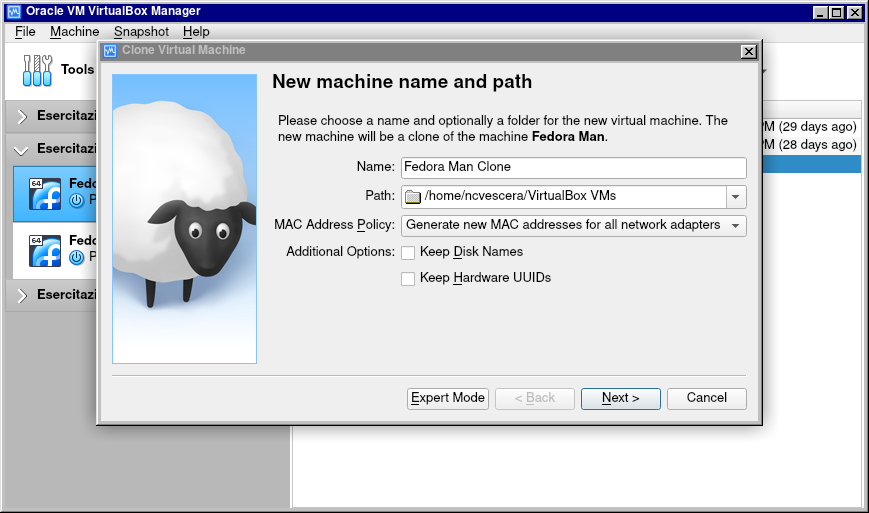
\includegraphics[width=\textwidth]{screens/vb_macpolicy.png}
\end{center}

\section{Configurazione Software}

\subsection{Sistema Operativo}

RIEMPIMI

\subsection{Software Necessario}

Appena ho terminato la fase di installazione del SO, ho provveduto ad aggiornarlo con i
seguenti comandi, per evitare problemi di compatibilit\`{a} e software obsoleto:

\begin{lstlisting}[style=cmd]
 sudo apt update
 sudo apt upgrade
\end{lstlisting}
\ \\
Poi ho installato i pacchetti necessari (\lstinline[style=cmd]|HTCondor| e \lstinline[style=cmd]|stress-ng|) con:

\begin{lstlisting}[style=cmd]
 sudo apt install htcondor 
 sudo apt install stress-ng
\end{lstlisting}
\ \\
Durante l'installazione del software \lstinline[style=cmd]|HTCondor| verr\`{a} si apre un menu dove mi viene chiesto se utilizzare una configurazione gi\`{a} pronta di Condor, io ho scelto \lstinline[style=cmd]|No| in quanto ho preferito configurare tutto a mano per comprendere meglio il file di configurazione ed i vari parametri da modificare.\\
\ \\
Il pacchetto \lstinline[style=cmd]|stress-ng| serve per mettere sotto sforzo i vari core della macchina e verr\`{a} utilizzato in seguito per testare la configurazione dei due slave.

\subsection{IP}

Ho assegnato IP statici alle macchine per essere sicuro di poterle sempre raggiungere e che
il DHCP del mio router non gli assegni indirizzi diversi col passare del tempo.\\
Gli indirizzi che ho scelto sono:
\begin{itemize}
	\item Master: 192.168.178.57
	\item Slave 1: 192.168.178.54
	\item Slave 2: 192.168.178.59
\end{itemize}
Per farlo ho utilizzato la seguente procedura (\`{e} uguale per tutte le macchine, basta solo cambiare l'ip):

\begin{enumerate}
	\item Ho creato il file \lstinline[style=cmd]|99-disable-network-config.cfg| e l'ho popolato con la seguente configurazione:
	
	\begin{lstlisting}[style=cmd]
 echo "network: {config: disabled}" | sudo tee /etc/cloud/cloud.cfg.d/99-disable-network-config.cfg
	\end{lstlisting}
	\item Ho riscritto il file di configurazione \lstinline[style=cmd]|/etc/netplan/00-installer-config.yaml| con:
	
	\begin{lstlisting}[style=cmd]
 network:
   version: 2
   renderer: networkd
   ethernets:
     enp0s3:
       dhcp4: no
       addresses:
         - 192.168.178.57/24
       gateway4: 192.168.178.1
       nameservers:
         addresses: [8.8.8.8, 1.1.1.1]
	\end{lstlisting}
	\item Ho riavviato la macchina per rendere effettive le modifiche.
\end{enumerate}

Per le altre macchine va modificato il parametro \lstinline[style=cmd]|addresses| con il corretto IP.\\
\ \\
Per controllare il corretto funzionamento di questa operazione basta utilizzare il comando \lstinline[style=cmd]|ifconfig enp0s3| e controllare che abbia il giusto indirizzo:

\begin{lstlisting}[style=output]
 enp0s3: flags=4163<UP,BROADCAST,RUNNING,MULTICAST>  mtu 1500
 inet 192.168.178.57  netmask 255.255.255.0  broadcast 192.168.178.255
 ...
\end{lstlisting}
 
 \subsection{hosts \& hostname}
 \label{sec:hosts}
 
 Ho modificato il file \lstinline[style=cmd]|/etc/hostname| definendo un nome diverso per ogni macchina in modo
 tale da poterle distinguere pi\`{u} facilmente durante le sessioni SSH:
 
 \begin{itemize}
 	\item Nome Macchina 1 (Master): \lstinline[style=cmd]|joemaster|
 	\item Nome Macchina 2 (Slave1): \lstinline[style=cmd]|joeslave1|
 	\item Nome Macchina 3 (Slave2): \lstinline[style=cmd]|joeslave2|
 \end{itemize} 
\ \\
In tutte le macchine, alla fine del file \lstinline[style=cmd]|/etc/hosts| ho aggiunto le seguenti righe per
facilitare poi la configurazione di htcondor:

\begin{lstlisting}[style=cmd]
 192.168.178.57	nodo1	nodo1.condor
 192.168.178.54	nodo2	nodo2.condor
 192.168.178.59	nodo3	nodo3.condor
\end{lstlisting}

\subsection{Firewall}

Per evitare problemi di comunicazione tra le varie macchine ho deciso di disabilitare il firewall.\\
In Ubuntu 20.4 LTS solitamente il firewall \`{e} disabilitato. Ho comunque controllato con il comando:

\begin{lstlisting}[style=cmd]
 sudo ufw status
\end{lstlisting}
\ \\
Se ho questo output vuol dire che il servizio non \`{e} attivo:

\begin{lstlisting}[style=output]
 Status: inactive
\end{lstlisting}
\ \\
In caso contrario lo andr\`{o} a disabilitare con:

\begin{lstlisting}[style=cmd]
 sudo ufw disable
\end{lstlisting}

\subsection{Configurazione HTCondor}